\documentclass[12pt]{article}
\usepackage{amsmath, amssymb, amsthm}
\usepackage{geometry}
\usepackage{graphicx}
\geometry{a4paper, margin=0.7in}
\usepackage[numbers]{natbib}

% Document metadata
\title{Physics of Open Quantum Systems: Explanation of Results}
\author{Rowan Adeya}
\date{\today}

\begin{document}

\maketitle

In this document, we shall attempt to explain the results from our QuTip simulations for two models: The Jaynes-Cummings Model and the {\textbf{[unknown model name]}}. For each model, we shall consider:
\begin{enumerate}
    \item Spontaneous Atomic Emission Decay Operator,
    \begin{equation}
        L = \gamma \hat{\sigma_-} \label{L_tls}
    \end{equation}
    \item QHO photon loss/gain Operator, 
        \begin{align}
            L = \gamma_0(N+1)\hat{a} \\ \label{L_qho}
            L = \gamma_0N\hat{a}^\dagger 
        \end{align}
    where 
    $N = [\exp{(\omega_c/k_BT)} -1]^{-1}$ is the mean number of quanta in the mode with frequency $\omega_c$.
    \item Both Operators together.
\end{enumerate}

It should also be noted that we are running the simulations under the resonance condition $\omega_a = \omega_c = \omega$. Furthermore, we are in the weak coupling regime, where $ g \ll \omega$, and that $g < \gamma,\gamma_0$ in order to observe the Rabi Oscillations. We are in a very low temperature regime, such that $N \approx 0$ and the cavity photon loss dominates. 

\section{Jaynes-Cummings Model (JCM)}

Recall the Hamiltonian for the Jaynes-Cummings Model:

\begin{equation}
    \hat{H} = \hat{H}_{TLS} + \hat{H}_{QHO} + \hat{H}_{int}, 
\end{equation} \label{JC_H}
where 
\begin{align*}
    \begin{aligned}
        \hat{H}_{TLS} &\equiv \frac{\hbar\omega_a}{2}\hat{\sigma}_z \\
        \hat{H}_{QHO} &\equiv \hbar\omega_ca^\dagger a \\
        \hat{H}_{int} &\equiv \hbar g(a\hat{\sigma}_{eg} + a^\dagger\hat{\sigma}_{ge}).
    \end{aligned}
\end{align*}

In \eqref{JC_H}, $\hbar\omega_a$ represents the energy of the photons emitted by the atom, $\hbar\omega_c$ the energy spacing between the QHO modes, and $g$ the coupling strength between the QHO and atom. In the interaction Hamiltonian $\hat{H}_{int}$, we can see that the QHO lowering operator $\hat{a}$is coupled to that of the atomic raising operator $\hat{\sigma}_{eg}$, and the QHO raising operator $\hat{a}^{\dagger}$ is coupled to that of the atomic lowering operator $\hat{\sigma}_{ge}$. 

This interaction term causes Rabi Oscillations (oscillatory transfers of energy between the atom and the QHO cavity), which we shall see are present in all of our results. As such, the only allowed states in the total state are $|g,n+1\rangle$ and $|e,n\rangle$.

For our simulation, we use the initial condition:

\begin{equation}
    |\Psi(0)\rangle = |e,n=2\rangle \label{init_e}
\end{equation}

The eigenvalues of the atom are $1 \rightarrow |e\rangle$ and $0 \rightarrow |g\rangle$, and so our expectation value for the TLS (atom excitation probability) lies between $0$ and $1$. The eigenvalues of the QHO are $n, n+1$, i.e. the eigenvalues of the number operator. We are considering $n=2$, so the expectation value of the TLS (cavity photon number) lies between $2 \rightarrow n$ and $3 \rightarrow n+1$ in closed systems, and in open systems, the maximum expectation value is $3 \rightarrow n+1$, since the system may decay to lower fock states.

\subsection{Spontaneous Atomic Emission}

\begin{figure}[h]
    \centering
    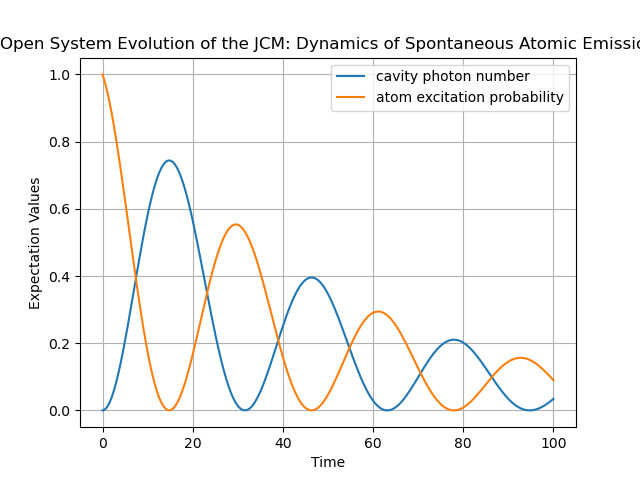
\includegraphics[width=\linewidth]{Research Project/Code/results/JCM/OQS_TLS_Decay.png}
    \caption{Plot of JCM evolution under spontaneous atomic decay.}
    \label{JCM_OQS_TLS}
\end{figure}

In this simulation, the atom starts in an excited state, and due to spontaneous atomic emission, we expect its state gradually over time to the ground state (since it cannot decay further). The cavity is confined to the $n=2$ fock space, and so we expect the expectation value of the cavity to be maximally $3$. Since The cavity and the atom are coupled by $H_{int}$, we expect to see Rabi Oscillations and exchange of energy (photons) and an eventual decay of the cavity mode due to the decaying atom. \\
\\
Figure \ref{JCM_OQS_TLS} clearly shows the TLS decaying over time, starting at the excited state (initial condition, expectation value = 1) and decaying to the ground state (expectation value = 0). Due to the JCM's coupling between the atom and cavity, we also see the expected decay of the cavity. The cavity starts at the initial fock state ($n=2$), and peaks at around $2.7$. This peak is not exactly $3$ because by the time the first half-period of the Rabi oscillations occur, the system has already lost energy to the reservoir via the $\hat{sigma_-}$ decay channel. It is further interesting to see that the peaks of the atom excitation coincide with the troughs of the cavity mode, as this displays the allowed states $|g,n+1\rangle$ and $|e,n\rangle$ which we expect. 

\subsection{Cavity Photon Gain/Loss}

\begin{figure}[h]
    \centering
    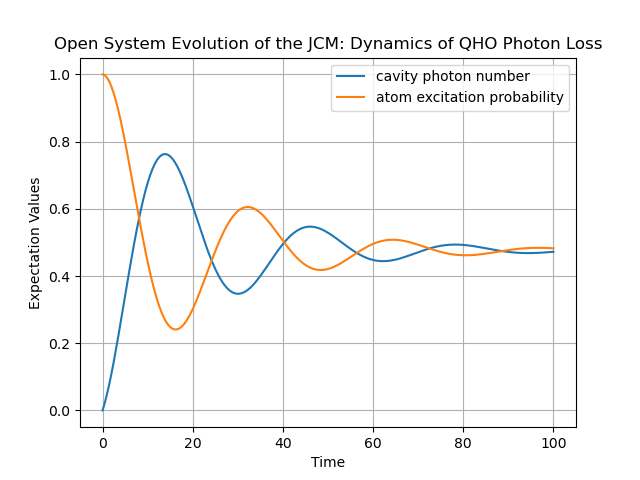
\includegraphics[width=\linewidth]{Research Project/Code/results/JCM/OQS_QHO_loss.png}
    \caption{Plot of JCM evolution under cavity photon loss/gain decay channel.}
    \label{JCM_OQS_QHO}
\end{figure}

In this simulation, the atom starts in an excited state, and due to cavity photon loss dominating (due to low temperature regime), we expect the cavity to decay over time to 0, with a starting initial fock state of $n=2$ and a maximum fock state of $n=3$. Due to $H_{int}$, we expect both Rabi oscillations and the atom to decay from excited state to ground state.

Figure \ref{JCM_OQS_QHO} again matches our expectations exactly. The cavity decays primarily through the dominant photon loss channel, starting at $n=2$ and decaying to 0. The cavity's expectation value is maximal around $n=2.5$ because the system has likely already lost energy to the reservoir. The atom also decays as expected, with the peaks of the atom coinciding again with the troughs of the cavity. The observed Rabi Oscillations, however, are much less pronounced than the Spontaneous Atomic Decay channel. This may be because the operator \eqref{L_qho} relies on a value of $N \approx 0$ in order to make photon loss dominant, but perhaps our choice of temperature is still too high for the JCM, and so $\gamma_0 (N+1) > \gamma$, which means that Rabi oscillations aren't pronounced (decay rates must be less than the coupling strength, and the larger that difference is, the more pronounced the Rabi oscillations are). 

\subsection{Spontaneous Atomic Emission and Cavity Photon Loss/Gain}

\begin{figure}[h]
    \centering
    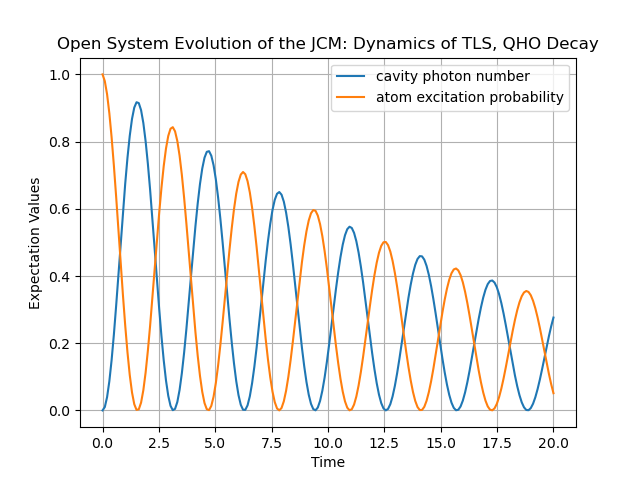
\includegraphics[width=\linewidth]{Research Project/Code/results/JCM/OQS_QHOTLS.png}
    \caption{Plot of JCM evolution under spontaneous atomic decay and cavity photon loss/gain channels.}
    \label{JCM_OQS_QHOTLS}
\end{figure}

In this simulation, the atom starts in an excited state, and due to cavity photon loss dominating and spontaneous atomic emission, we expect the cavity to decay over time to 0 and the atom to decay from excited to ground state, with a starting initial fock state of $n=2$ and a maximum fock state of $n=3$, and the atom starting at an excited state. Due to $H_{int}$, we expect both Rabi oscillations and the atom to decay from excited state to ground state. Moreover, we expect the atom and cavity both to decay much faster because both decay channels are active, instead of one or the other. 

Figure \ref{JCM_OQS_QHO} again matches our expectations exactly. The cavity and atom both decay due to the respective channels and the $H_{int}$ coupling. The Rabi oscillations are even less pronounced than in Figure \ref{JCM_OQS_QHO}, likely because we have both decay rates acting on the individual subsystems, leading to the total effect of bringing the total system decay rate closer to the coupling strength. Furthermore, both the maximum expectation of the cavity and the minimum expectation value for the cavity at the first half-period peak of the Rabi oscillations are lower/higher than expected, likely due to the rapid rate at which the system is decaying due to both channels being open. The system decays in $\approx 500 \frac{\hbar}{\omega}$ seconds, compared to just the cavity decay channel which decays at around $\approx 1000 \frac{\hbar}{\omega}$ seconds. Again, this is due to both decay channels being open.

\section{Exciton--Vibration Model}

The Hamiltonian for the Exciton--Vibration Model is (noting $\hbar = 1$):

\begin{equation}
    \hat{H} = \hat{H}_{TLS} + \hat{H}_{QHO} + \hat{H}_{int}, 
\end{equation} \label{EV_H}
where 
\begin{align*}
    \begin{aligned}
        \hat{H}_{TLS} &\equiv \frac{\Delta\epsilon}{2}\hat{\sigma}_z + V\sigma_x \\
        \hat{H}_{QHO} &\equiv \omega_ca^\dagger a \\
        \hat{H}_{int} &\equiv -\frac{g}{\sqrt{2}}\sigma_z \otimes(a^\dagger + a).
    \end{aligned}
\end{align*}

$\Delta\epsilon$ refers to the energy difference between the TLS levels, and $V$ is the tunnelling amplitude. \\
\\
This Hamiltonian causes oscillations in both the TLS and QHO subsystems. If we look at the action of, say, the Hamiltonian on the state $|e\rangle$, the interaction Hamiltonian does not change the TLS state. In fact, the free TLS Hamiltonian does so, with the term $V\sigma_x$ being responsible for the TLS oscillations. 
In order to see what may happen for the QHO subsystem, it is convenient to set $V=0$ such that the TLS is simply a constant factor. In this case, the Hamiltonian may look like:

\begin{equation*}
    \hat{H} = \omega a^\dagger a - \frac{g}{\sqrt{2}}(a + a^\dagger) \rightarrow \hat{H} = \omega(b^\dagger b - k)
\end{equation*}

where $b = a - \frac{g}{\sqrt{2}} $ is the annihilation operator with a displacement, and $k = \frac{g}{\sqrt{2}\omega}$. This new form is a displaced Harmonic Oscillator, which implies that the QHO does indeed oscillate. 

In terms of physical parameters, we use data from \cite{ExVib2014-Hamiltonian}, which is measured in cm$^{-1}$ frequency. Moreover, we note that we are in a room temperature regime ($\approx300 K$), which is reflected in the QHO photon gain/loss parameter.  

\vspace{5cm}
\begin{center}
    {\Large{*        *        *}}
\end{center}
\newpage


\subsection{Spontaneous Atomic Emission}

\begin{figure}[h]
    \centering
    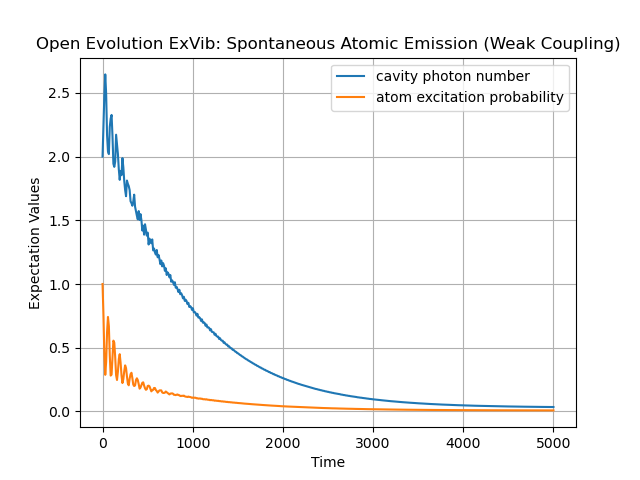
\includegraphics[width=\linewidth]{Research Project/Code/results/ExVib/OQS_TLS_Decay.png}
    \caption{Plot of EV evolution under spontaneous atomic decay.}
    \label{ExVib_OQS_TLS}
\end{figure}

In this simulation, the atom starts in an excited state, and due to cavity photon loss dominating (due to low temperature regime), we expect the cavity to decay over time to 0, with a starting initial fock state of $n=2$.

We see that both the TLS and QHO decay to their lowest states ($|g\rangle, |0\rangle$ respectively). 
The TLS, due to the $V\sigma_x$ term, oscillates between the excited and ground states. The decay channel $L = \gamma|g\rangle\langle e|$ however, decays the TLS population into the ground state. If, for example, $V = 0$, then there would still be decay from $|e\rangle \rightarrow |g\rangle$. However, if the TLS subsystem starts in $|g\rangle$, the system will never populate $|e\rangle$ due to the $\sigma_x$ term not being present and thus not causing oscillations between the two levels. 
The QHO is also indirectly influenced by the $V\sigma_x$ term


\subsection{Cavity Photon Gain/Loss}

\begin{figure}[h]
    \centering
    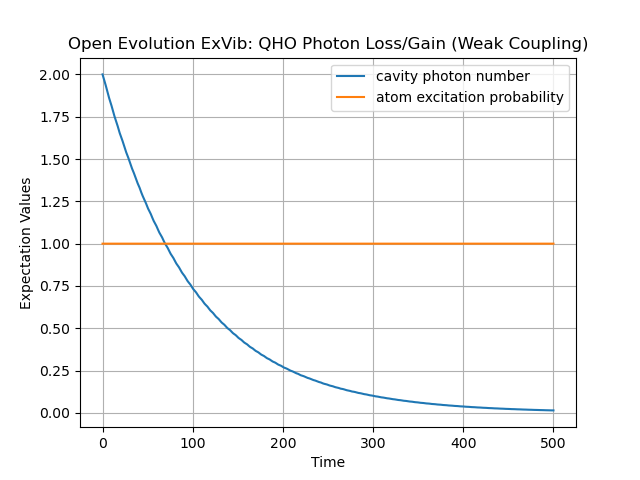
\includegraphics[width=\linewidth]{Research Project/Code/results/ExVib/OQS_QHO_loss.png}
    \caption{Plot of EV evolution under cavity photon gain/loss.}
    \label{ExVib_OQS_QHO}
\end{figure}

\subsection{Spontaneous Atomic Emission and Cavity Photon Loss/Gain}

\begin{figure}[h]
    \centering
    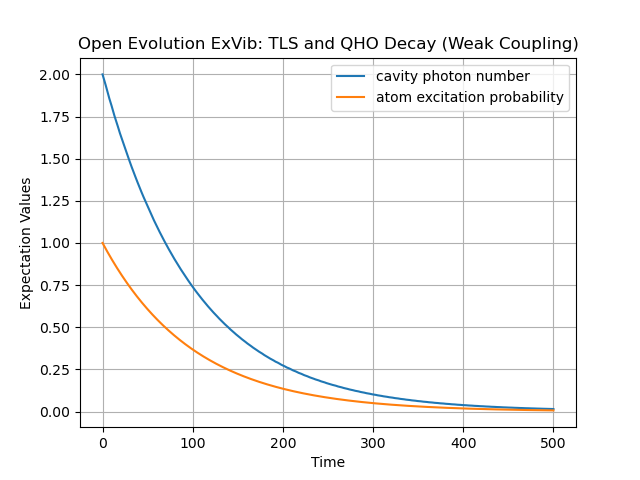
\includegraphics[width=\linewidth]{Research Project/Code/results/ExVib/OQS_QHOTLS.png}
    \caption{Plot of EV evolution under spontaneous atomic decay and cavity photon loss/gain channels.}
    \label{EV_OQS_QHOTLS}
\end{figure}



\newpage

\bibliographystyle{unsrt} 
\bibliography{References/references.bib} 
\end{document}
